\documentclass[aspectratio=169]{beamer}

\mode<presentation>{
  \usetheme{Boadilla}
}
\definecolor{lmugreen}{RGB}{0, 136, 58}
\usecolortheme[named=lmugreen]{structure}

\usepackage[T1]{fontenc}
\usepackage[utf8]{inputenc}
\usepackage{graphicx}
\usepackage{booktabs}

\title[Joint Model Importance]{Joint Model Importance via the Rashomon Set}
\subtitle{Behavioural Comparison of Near-Equally-Good Models}
\author{Fiona K.~Ewald}
\institute[LMU/MCML]{LMU Munich \,\textbullet\, MCML}
\date{\today}

\titlegraphic{%
  
\includegraphics[height=1.4cm]{../logos/lmu.png}\hspace{2em}%
  
\includegraphics[height=1.4cm]{../logos/mcml.jpg}%
}

\begin{document}

% -----------------------------------------------------------------
\begin{frame}
  \titlepage
\end{frame}

% -----------------------------------------------------------------
\begin{frame}{Beyond the single best model}
  \begin{itemize}
    \item In tabular ML, many models reach indistinguishable predictive performance.
    \item The \emph{Rashomon set}
      \(
        \mathcal{R}_\varepsilon \;=\; \bigl\{\, m \,:\, \mathrm{score}(m) \le \mathrm{score}(m^{*}) \cdot (1 + \varepsilon) \,\bigr\}
      \)
      collects every model within $\varepsilon$ of the best.
    \item Members of $\mathcal{R}_\varepsilon$ can disagree substantially on individual predictions and on feature importance.
    \item \textbf{Question.} How are these equally good models related to one another, and what does the collective tell us beyond the single best?
  \end{itemize}
\end{frame}

% -----------------------------------------------------------------
\begin{frame}{Pipeline}
  \begin{enumerate}
    \item For every $m \in \mathcal{R}_\varepsilon$, compute predictions on a held-out 2/3 validation split.
    \item Build the pairwise \emph{behavioural distance} matrix
      \( d_{ij} \;=\; \|\hat y_i - \hat y_j\|_p \).
    \item View the matrix three ways:
      \begin{itemize}
        \item hierarchical clustering (\texttt{hclust})
        \item classical MDS (\texttt{cmdscale}, $k = 2$)
        \item partitioning around medoids (\texttt{cluster::pam})
      \end{itemize}
  \end{enumerate}
  \vspace{1ex}
  \footnotesize Predictions are class probabilities for classification, $\hat y$ for regression. Distances computed for both Euclidean and Manhattan; results shown are Euclidean (Manhattan tells the same story).
\end{frame}

% -----------------------------------------------------------------
\begin{frame}{Setup}
  Rashomon tolerance $\varepsilon = 1\%$ of the best score.\\
  Five learner families considered for every task: \texttt{tree}, \texttt{glmnet}, \texttt{xgb}, \texttt{nnet}, \texttt{svm}.
  \vspace{2ex}
  \begin{table}[h]
    \centering
    \begin{tabular}{lll}
      \toprule
      Key & Task & Type \\
      \midrule
      \texttt{gc} & German Credit  & classification \\
      \texttt{cs} & COMPAS         & classification \\
      \texttt{bs} & Bike Sharing   & regression     \\
      \texttt{st} & Synthetic      & regression     \\
      \bottomrule
    \end{tabular}
  \end{table}
\end{frame}

% -----------------------------------------------------------------
\begin{frame}{Who survives the Rashomon cut?}
  \begin{table}[h]
    \centering
    \begin{tabular}{ll}
      \toprule
      Task & Surviving families ($n$ models) \\
      \midrule
      \texttt{gc} & \texttt{svm}\,(9), \texttt{xgb}\,(125) \\
      \texttt{cs} & \texttt{nnet}\,(15), \texttt{tree}\,(261) \\
      \texttt{bs} & \texttt{tree}\,(30) \\
      \texttt{st} & \texttt{nnet}\,(216), \texttt{svm}\,(160) \\
      \bottomrule
    \end{tabular}
  \end{table}
  \vspace{1ex}
  \textbf{First finding.} At $\varepsilon = 1\%$ only one or two learner families survive per task --- \emph{learner choice} is the first dimension of disagreement inside $\mathcal{R}_\varepsilon$.
\end{frame}

% -----------------------------------------------------------------
\begin{frame}{MDS view --- all four tasks}
  \centering
  \begin{tabular}{@{}c@{\hspace{1ex}}c@{}}
    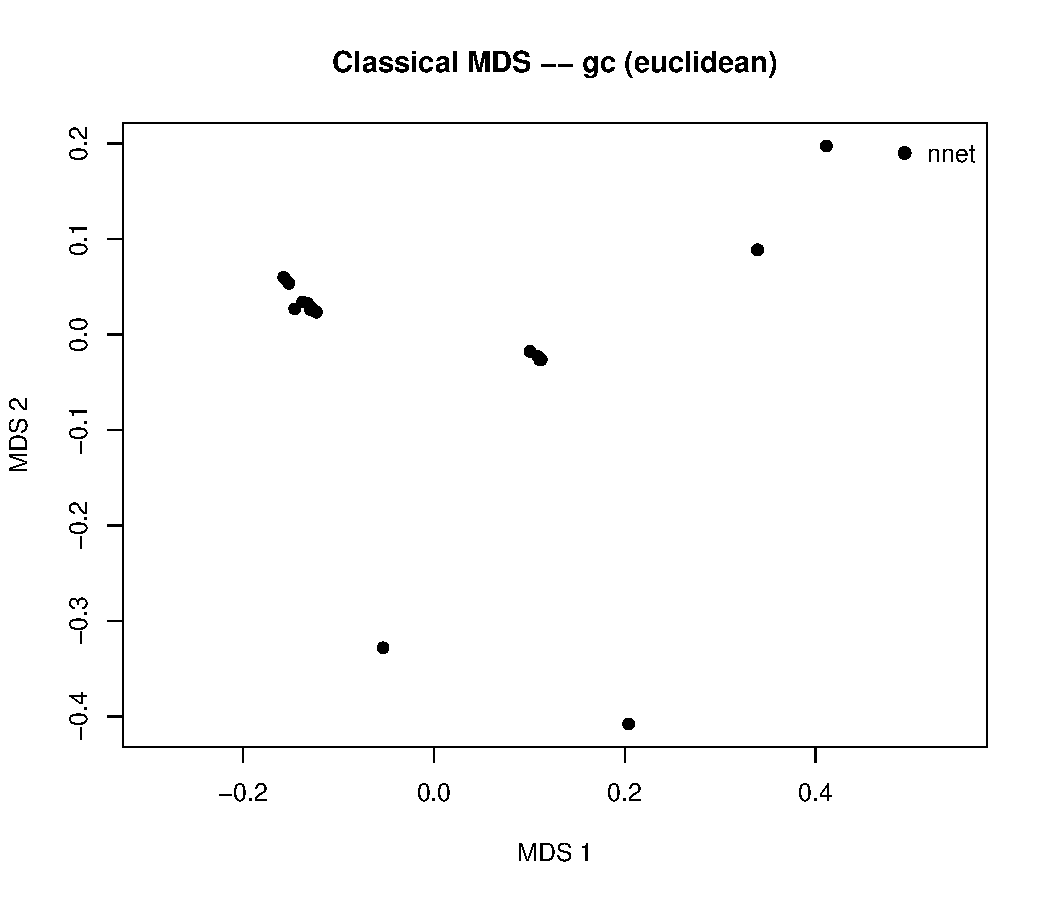
\includegraphics[height=0.4\textheight,keepaspectratio]{../figures/mds_gc_euclidean.pdf} &
    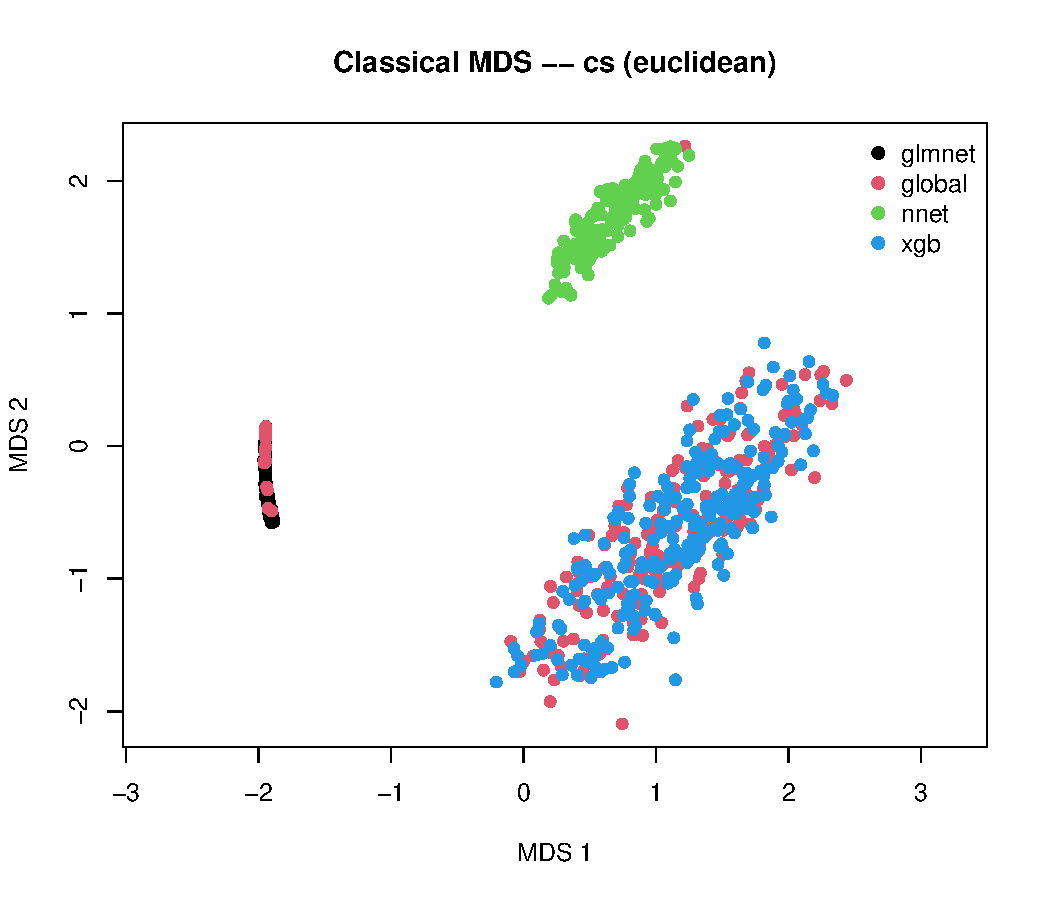
\includegraphics[height=0.4\textheight,keepaspectratio]{../figures/mds_cs_euclidean.pdf} \\[-1ex]
    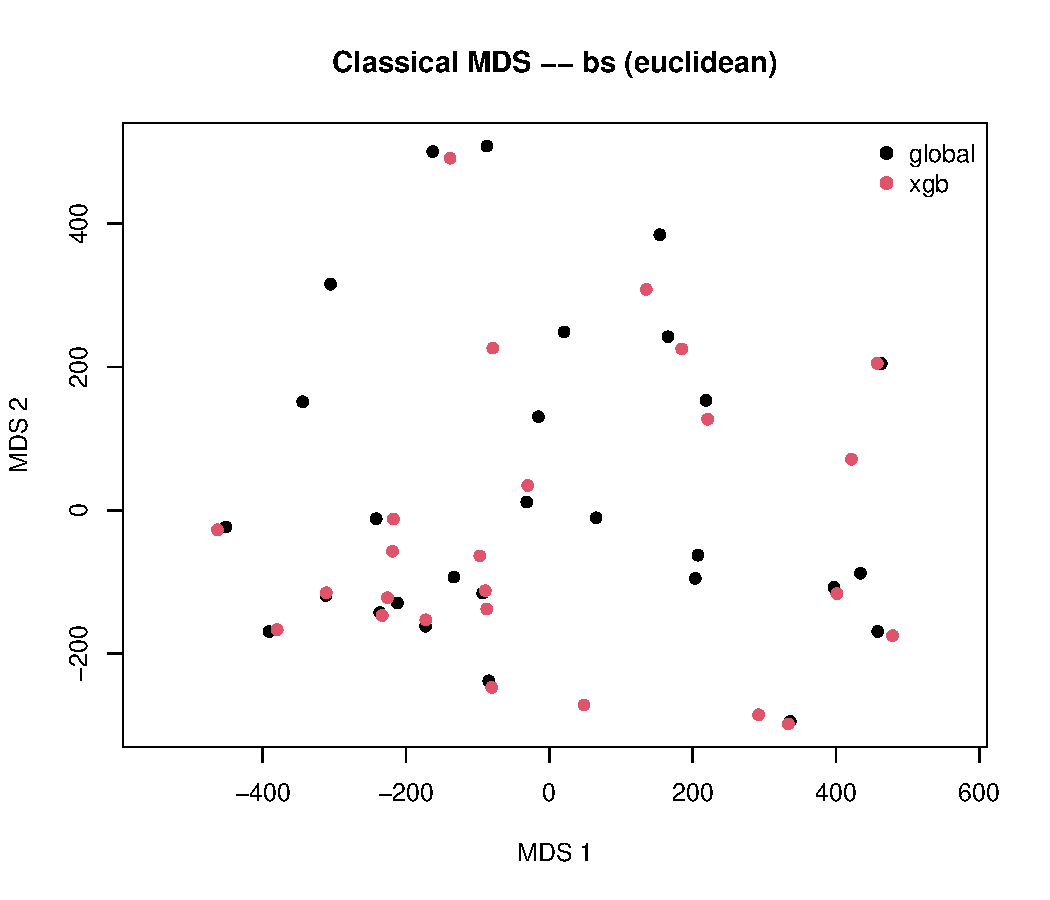
\includegraphics[height=0.4\textheight,keepaspectratio]{../figures/mds_bs_euclidean.pdf} &
    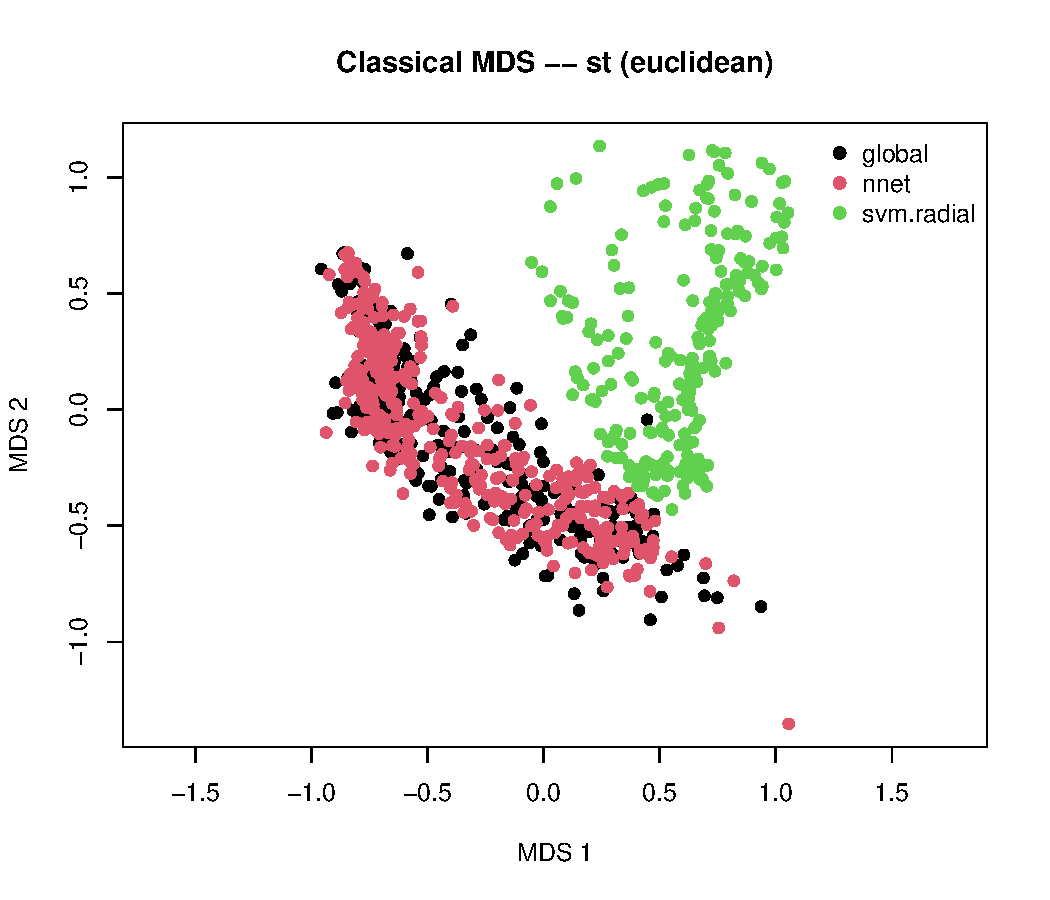
\includegraphics[height=0.4\textheight,keepaspectratio]{../figures/mds_st_euclidean.pdf}
  \end{tabular}
\end{frame}

% -----------------------------------------------------------------
\begin{frame}{Reading the MDS plots}
  \begin{itemize}
    \item Wherever two families coexist, behavioural distance \textbf{separates them cleanly} --- the dominant axis is family identity, not within-family variation.
    \item Within-family variance is \emph{asymmetric}: \texttt{svm} and \texttt{nnet} form tight clusters; \texttt{tree} and \texttt{xgb} scatter widely despite fewer tunable hyperparameters.
    \item Several families trace out a \textbf{1D-manifold} in the MDS plane (e.g.\ \texttt{st}/\texttt{nnet}, \texttt{cs}/\texttt{tree}) --- next two slides.
  \end{itemize}
\end{frame}

% -----------------------------------------------------------------
\begin{frame}{Within-family structure I --- \texttt{st}\,/\,\texttt{nnet}}
  \centering
  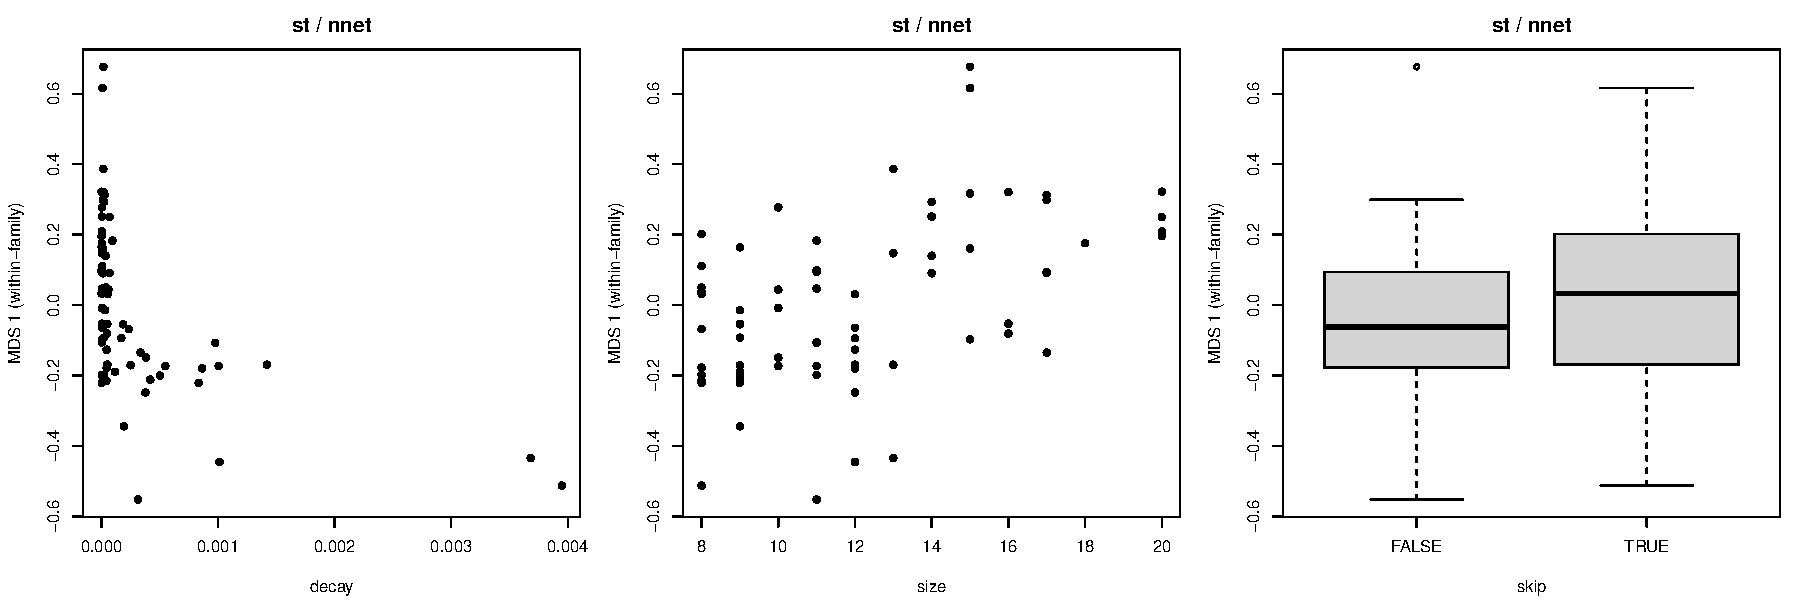
\includegraphics[width=0.95\textwidth,height=0.55\textheight,keepaspectratio]{../figures/hp_trajectories/hp_vs_mds1_st_nnet.pdf}\\[0.5ex]
  \footnotesize
  \begin{itemize}
    \item Each panel: 1D within-family MDS coordinate vs.\ one hyperparameter.
    \item The within-family manifold \textbf{is the \texttt{decay} axis} --- near-monotone mapping.
    \item \texttt{size} and \texttt{skip} have no effect on behavioural position.
  \end{itemize}
\end{frame}

% -----------------------------------------------------------------
\begin{frame}{Within-family structure II --- \texttt{cs}\,/\,\texttt{tree}}
  \centering
  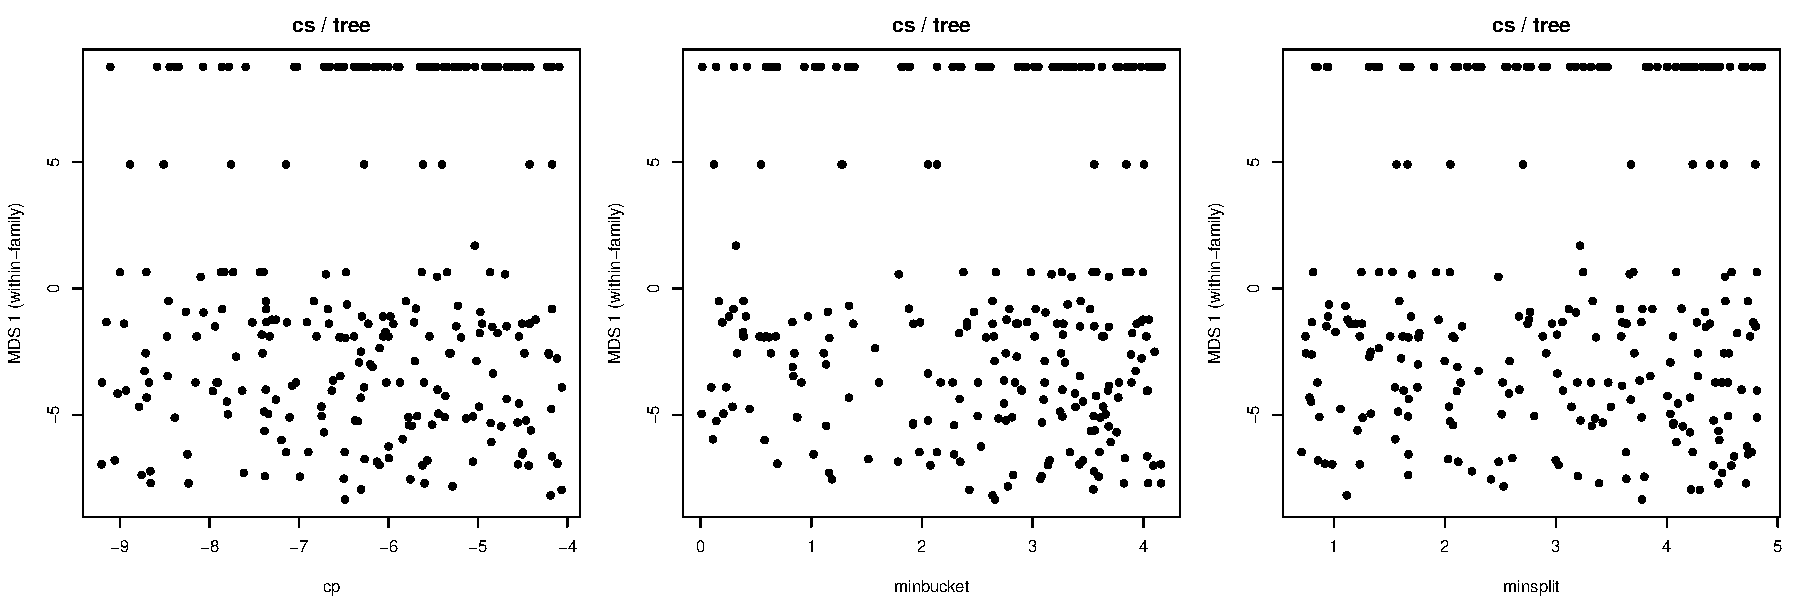
\includegraphics[width=0.95\textwidth,height=0.55\textheight,keepaspectratio]{../figures/hp_trajectories/hp_vs_mds1_cs_tree.pdf}\\[0.5ex]
  \footnotesize
  \begin{itemize}
    \item Within-family MDS coordinate vs.\ \texttt{cp}, \texttt{minbucket}, \texttt{minsplit}.
    \item Trees on COMPAS are \textbf{bimodal}: a tight cluster at MDS\,1 $\approx 8$ and a diffuse population below zero.
    \item \emph{No single tuned hyperparameter} separates the two modes --- a discrete behavioural split that tuning alone does not reach.
  \end{itemize}
\end{frame}

% -----------------------------------------------------------------
\begin{frame}{First interpretation}
  \begin{itemize}
    \item \textbf{Joint model importance is a two-level question:}
      \begin{enumerate}
        \item Which learner family does the model come from?
        \item Where on the family's behavioural manifold does it sit?
      \end{enumerate}
    \item Across every task observed, learner choice is the first axis of disagreement --- not hyperparameter setting.
    \item Within-family structure can be smooth and HP-aligned (\texttt{st}/\texttt{nnet} $\sim$ \texttt{decay}) or discrete and HP-orthogonal (\texttt{cs}/\texttt{tree}).
  \end{itemize}
\end{frame}

% -----------------------------------------------------------------
\begin{frame}{Next steps}
  \begin{itemize}
    \item \textbf{$\varepsilon$ sensitivity.} How does family composition shift as the Rashomon tolerance opens?
    \item \textbf{Feature-importance distance.} Compare behavioural distance with a distance built from VIC --- do the clusters agree?
    \item \textbf{Choose $k$ for PAM via silhouette}, then read out the medoids as ``representative'' members of the Rashomon set.
    \item \textbf{Disagreement map.} Where in feature space do Rashomon-set models disagree the most?
    \item \textbf{Discrete tree mode on \texttt{cs}.} Is the bimodality driven by structural differences (root split, depth) that hyperparameters do not capture?
  \end{itemize}
\end{frame}

% -----------------------------------------------------------------
\begin{frame}
  \centering \vfill
  {\Huge Thank you.}\\[1em]
  {\Large Questions?}
  \vfill
\end{frame}

\end{document}
